\chapter{%
実験}

RGB-Dカメラから取得したデータセットをRXDネットワークを使用し曲管又はT字管を認識できるか検証する。
物体認識においては他のネットワークでも実験し、RXDネットワークの有用性を確かめる。

\section{評価指標}
物体認識の評価指標ではパラメータ数(Params), Intersection over Union(IoU), mean Average Precision(mAP)を用い認識ネットワークの性能評価を行う。
まず、パラメータ数は認識ネットワークの学習可能なパラメータの合計数を示す。これにより、認識ネットワークの複雑度を示すことができる。
次に。IoUは正解と予測のバウンディングボックスの共通の重なり部分を2つのバウンディングボックスを重ねたときの総面積で除算したものである。
IoUは0~1.0の値の範囲で示され、値が大きければ大きいほどラベル付されたボックスと予測されたボックスの重なりが正しいことになり、正確に認識していると判断できる。
次に、mAPは1つ1つのクラスに対して平均適合率であるAP(Average Precision)を計算する。まず、モデルの予測結果を、出力する信頼度スコア順に並べる。
ラベルごとに信頼度スコアがそのラベルの値以上の予測結果について、適合率と再現率を求める。適合率と再現率は図4.1のようにTrue Positive(TP)とFalse Negative(FN)を用いて表される。
その適合率と再現率のグラフから適合率の下側の面積を求める。ここで、予測されたラベルが正解なのかの判断はIoUが決められたしきい値以上で、最も信頼度スコアが高い予測ラベルが正解とするように判断される。
そして最後に、クラスごとに計算されたAPの平均を算出したものがmAPになる。

\begin{figure}[htbt]
	\centering
	 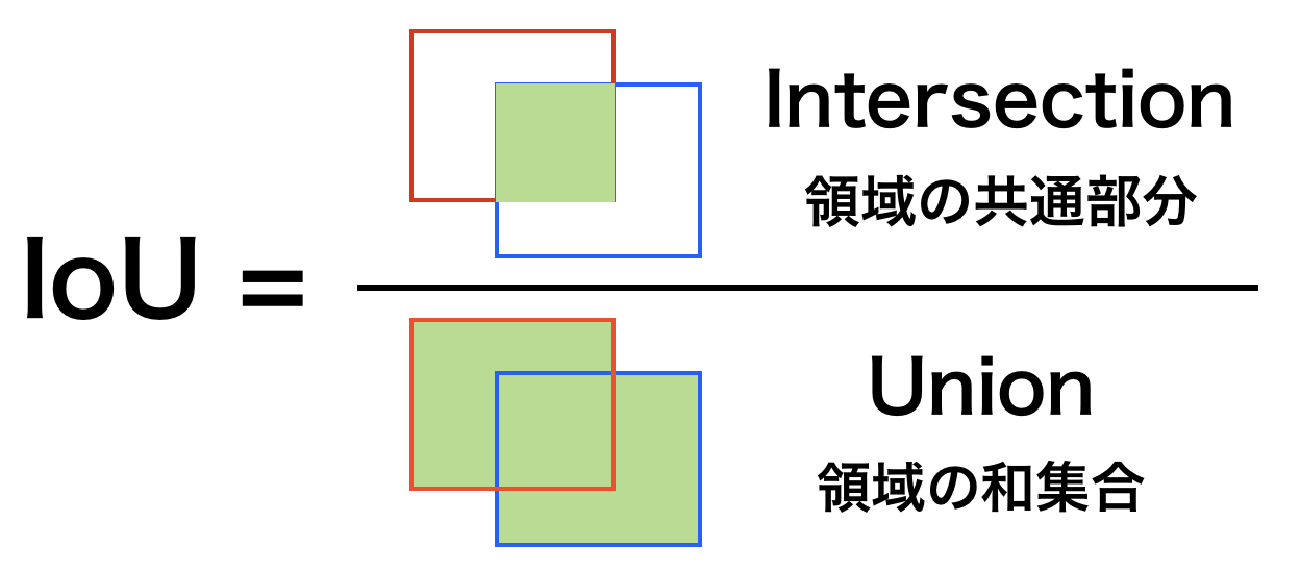
\includegraphics[height=45mm]{iou.eps}
	 \caption{Intersection over Union(IOU)}
	 \label{fig:f2}
\end{figure}

\begin{figure}[htbt]
	\centering
	 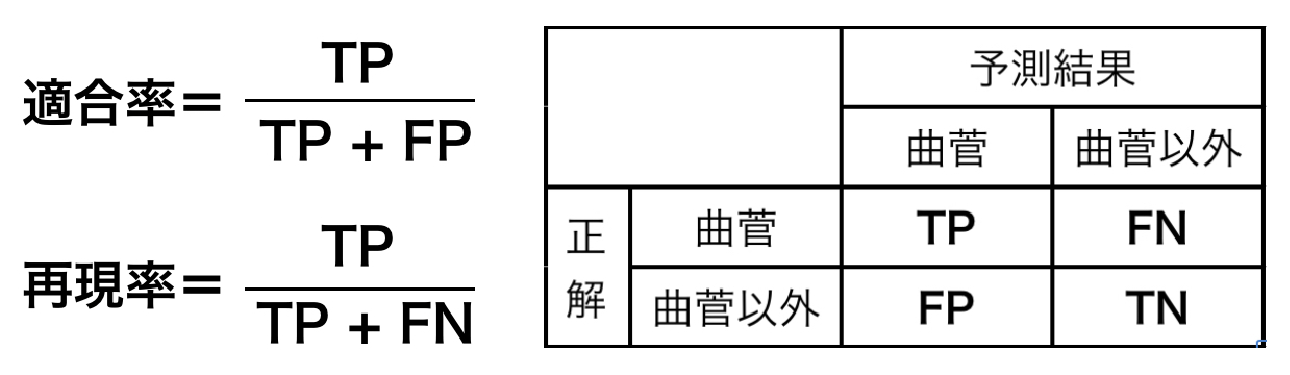
\includegraphics[height=35mm]{recall.eps}
	 \caption{適合率と再現率}
	 \label{fig:f2}
\end{figure}


\section{結果と考察}

\begin{table}[htbp]
\centering
\caption{物体検出ネットワークの実行結果}
\resizebox{\textwidth}{!}{%
\begin{tabular}{llllllll}
\hline
	\textit{\textbf{}} & \textit{\textbf{}} & \textit{\textbf{AP}} & \textit{\textbf{}} & \textit{\textbf{}} & \textit{\textbf{AP50}} & \textit{\textbf{}} & \textit{\textbf{Parameters}} \\
\textit{\textbf{Network}} & \textit{\textbf{bent}} & \textit{\textbf{junction}} & \textit{\textbf{all}} &  \textit{\textbf{bent}} & \textit{\textbf{junction}} & \textit{\textbf{all}} & \textit{\textbf{}} \textit{\textbf{millions}} \\ \hline
YOLOV3              & 33.9                 & 68.6                                 & 51.3                      & 9.95                      & 20.1                          & 15.0                     & 61.5                                \\
YOLOV3-Depth        & 1.3                  & 0.0                                 & 0.7                      & 0.4                      & 0.0                          	& 0.2                     & 86.3                                	\\
RXD                 & 70.9                 & 37.2                                 & 54.1                      & 20.8                      & 10.9                          & 15.8                     & 32.4                                 \\
\end{tabular}%
}
\end{table}

\begin{figure}[htbt]
	\centering
	 \includegraphics[height=85mm]{detect.eps}
	 \caption{適合率と再現率}
	 \label{fig:f2}
\end{figure}

\begin{figure}[htbt]
	\centering
	 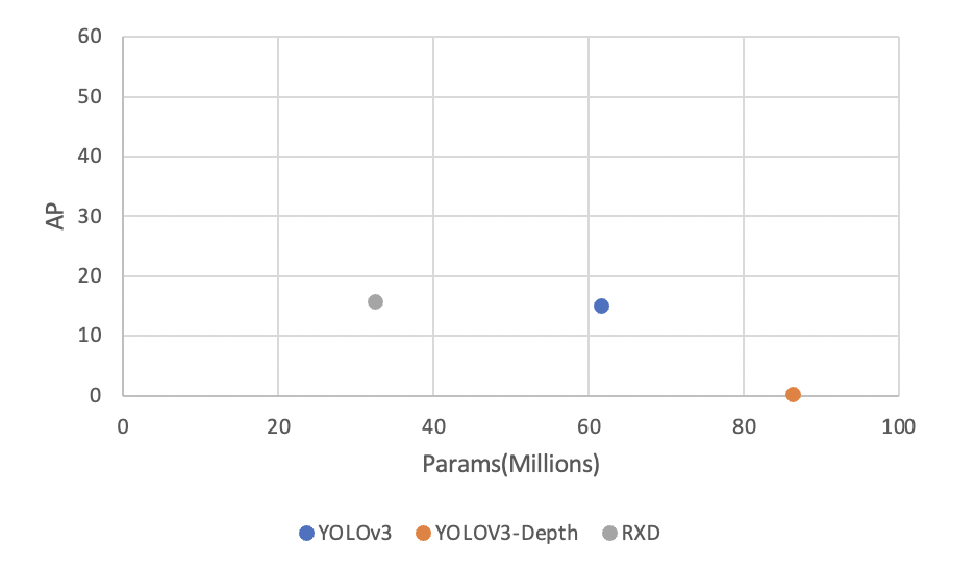
\includegraphics[height=85mm]{ap.eps}
	 \caption{適合率と再現率}
	 \label{fig:f2}
\end{figure}

\begin{figure}[htbt]
	\centering
	 \includegraphics[height=85mm]{ap50.eps}
	 \caption{適合率と再現率}
	 \label{fig:f2}
\end{figure}

表4.1よりRXDネットワークがAPとAP50の平均値がともに最も数値が高かった。また、パラメータ数に関してはYOLOv3, YOLOv3-Depthよりも低い値となりより優れているネットワークであると言える。
RGB画像だけでなくDepth画像も学習させると情報量が多くなるため、畳み込む回数も増加しパラメータ数が結果的に多くなる。しかし、RXDネットワークはパラメータ数を抑えつつ、優れた精度を持っているため実験したネットワークの中で最も良いネットワークであると言える。
しかし、APの平均値はともに優れた値であったが、bentとjunction個々の値で見るとYOLOv3のほうがjunctionを検出するにおいてはいい結果になっていた。そのため、認識したい物体によってはネットワーク検出器を変更することで、より望ましい結果を得られる可能性もある。
評価はAPとAP50で行ったが、APのほうが数値が低い結果となった。これはIoUの閾値を上昇させることで認識する条件を厳しくしているため、IoU閾値を増加させても認識精度が低くならない結果が望ましい。RXDネットワークはAPの値はAP50よりも大きく劣っているため、
ネットワーク改善を行う必要があると言える。


\begin{table}[htbp]
\centering
\caption{テスト画像を用いた検出結果}
\resizebox{\textwidth}{!}{%
\begin{tabular}{llllllll}
\hline
	\textit{\textbf{}} & \textit{\textbf{}} & \textit{\textbf{AP}} & \textit{\textbf{}} & \textit{\textbf{}} & \textit{\textbf{AP50}} & \textit{\textbf{}} & \textit{\textbf{Parameters}} \\                              \\
\end{tabular}%
}
\end{table}
図4.2の結果にそれぞれのネットワークの出力画像を示した。結果よりRXDネットワークが最も良い検出を示している。しかし、RXDネットワークの出力されたデータではT字管を認識できていない結果も存在している。
これは、もとのDepth画像のデータセットと比較すると遠くの物体になるほどデータが欠落しているため、認識が困難であったと考えられる。そのため、RGB-Dカメラの精度が低いと物体検出の精度に影響してくることがわかる。
また、暗闇の中でのテスト画像ではYOLOv3-DepthとRXDネットワークの出力結果が配管を認識できていた。これは暗闇の状況下でも影響を受けないDepth画像が役に立っていると考えられる。

\begin{figure}[htbt]
	\centering
	 \includegraphics[height=80mm]{6d.eps}
	 \caption{適合率と再現率}
	 \label{fig:f2}
\end{figure}


\begin{figure}[htbt]
	\centering
	 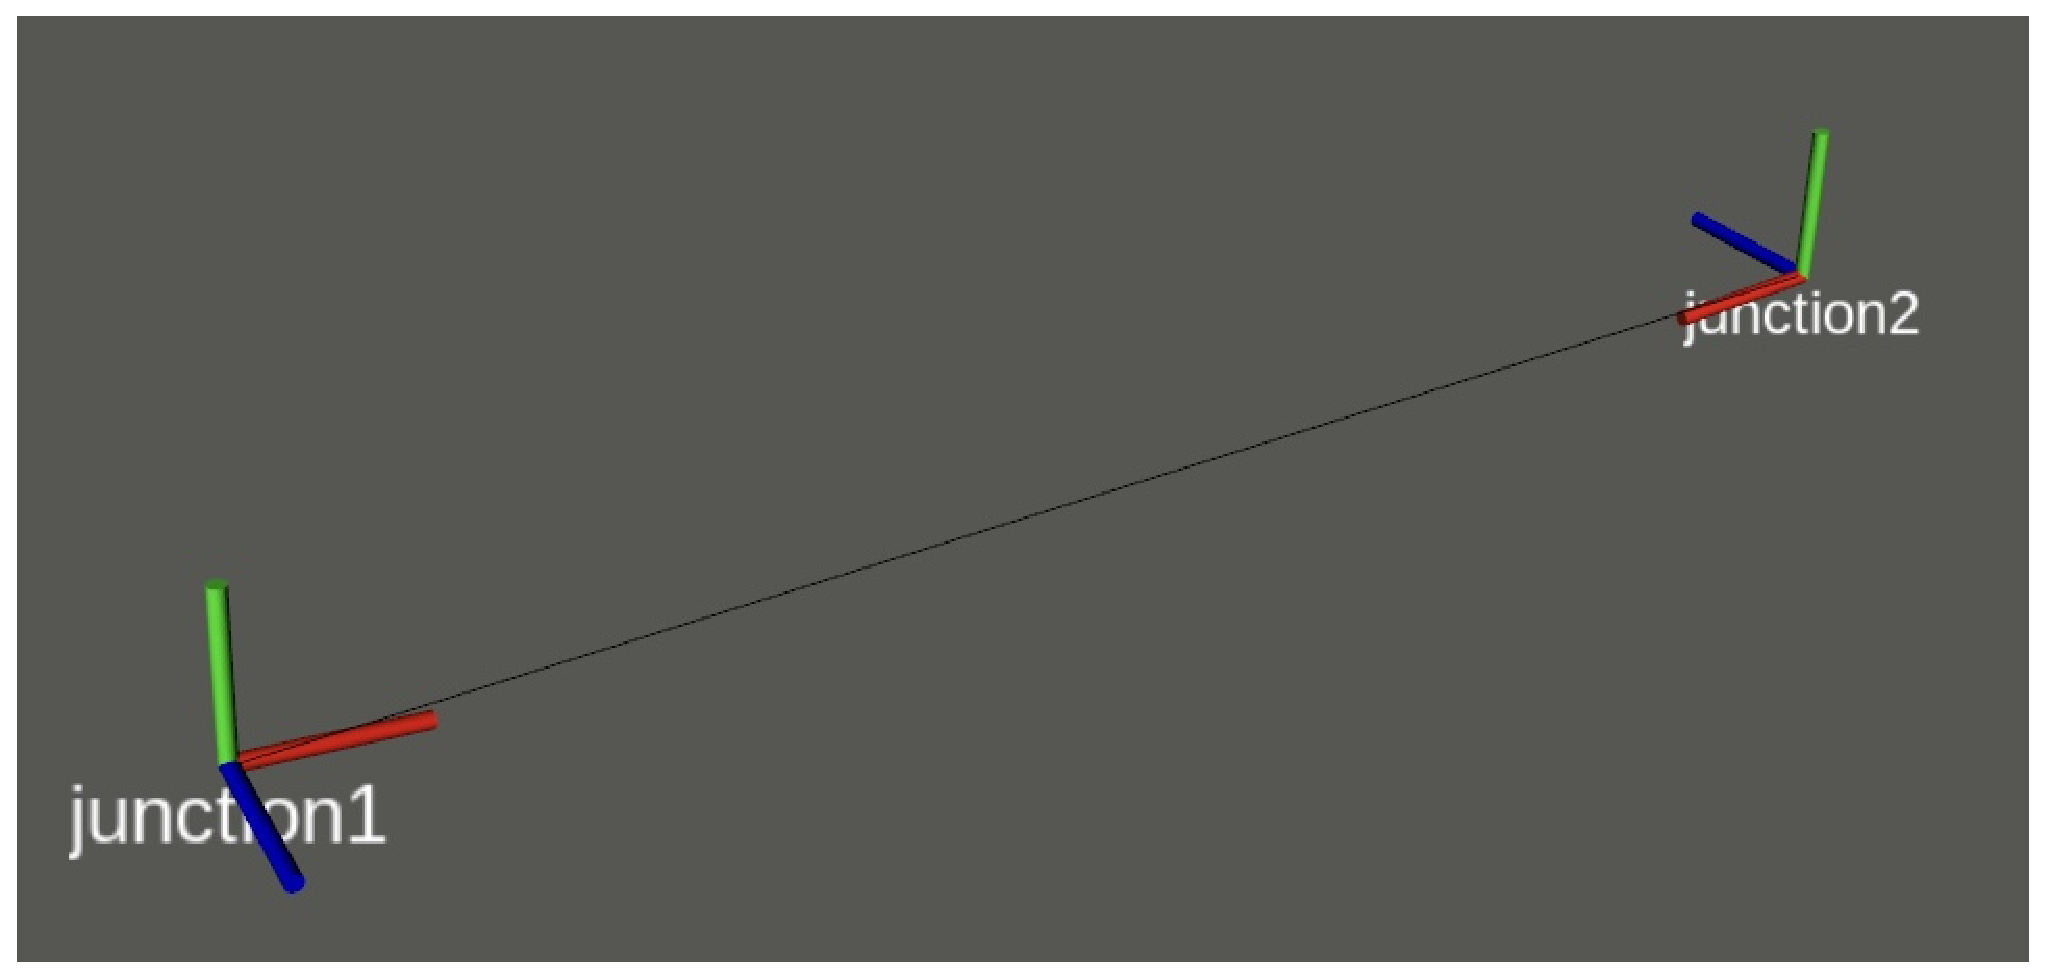
\includegraphics[height=65mm]{rviz.eps}
	 \caption{適合率と再現率}
	 \label{fig:f2}
\end{figure}

次に、6D姿勢推定の結果を図4.3に示す。既存のGen6Dのみでは検出器がオブジェクトの複数認識に対応していなかった。RXDネットワークは画像の中の全てのオブジェクトを認識可能なため、検出された値をGen6DのSelectorに渡すことで複数姿勢推定を可能とする。
しかし、結果では曲管の姿勢がボックスとうまく一致しなく望ましくない結果になった。
また、図4.4のようにjunction同士が向かい合っている画像の姿勢推定を行い、それぞれのオブジェクトのYaw, Pitch, Rollを求めた。表の結よりjunction同士が向かい合っていることがわかる。
次に、表の結果のそれぞれの姿勢を用いて、Rvizを使用してそれぞれのオブジェクトの座標系を可視化した。完全に向かい合った結果にはならなかったが、T字管の位置関係と姿勢を表示することができた。
